%!TEX program = xelatex
% 完整编译: xelatex -> biber/bibtex -> xelatex -> xelatex
\documentclass[lang=cn,11pt,a4paper]{elegantpaper}

\title{有限元第四次编程作业}
\author{W Huang}
\date{\zhtoday}


% 本文档命令
\usepackage{array}
\usepackage{float}
\usepackage{multirow}
\usepackage{amsmath}
\usepackage{amssymb}
\newcommand{\ccr}[1]{\makecell{{\color{#1}\rule{1cm}{1cm}}}}

\begin{document}

\maketitle

\section{Stokes方程}

\subsection{求解设置}

求解无滑移边界条件的不可压 Stokes 方程: 
\begin{equation}
    \left\{
        \begin{array}{ll}
            -\Delta \mathbf{u}+\nabla p = \mathbf{f}& ,\text{in}\;\Omega,\\
            \nabla\cdot \mathbf{u}& ,\text{in}\;\Omega,\\
            \mathbf{u} = 0& ,\text{on}\;\partial \Omega.
        \end{array}
    \right.
\end{equation}
可以导出弱形式: 
\begin{equation}
    (\nabla \mathbf{u},\nabla \mathbf{v}) 
    + (\nabla\cdot \mathbf{v},\nabla p)
    + (\nabla\cdot \mathbf{u},\nabla q)
    = (\mathbf{f},\mathbf{v}),\quad \forall \mathbf{v}\in H_0^1(\Omega),q\in L_0^2(\Omega).
\end{equation}
这里
\begin{equation}
    L_0^2(\Omega)=\left\{q\in L^2(\Omega):\int_\Omega q\;dx=0\right\}.
\end{equation}
现在我们在有限元空间 $\mathcal{P}_2^d\times \mathcal{P}_1$ 中取逼近. 
得到下述形式的离散线性系统:
\begin{equation}
    \begin{pmatrix}
        A_1 & O & B_1 \\
        O & A_2 & B_2 \\
        B'_1 & B'_2 & O
    \end{pmatrix}
    \begin{pmatrix}
        u_1\\
        u_2\\
        p
    \end{pmatrix}
    =
    \begin{pmatrix}
        f_1\\
        f_2\\
        0
    \end{pmatrix}.
\end{equation}
为方便起见, 我们下面记
\begin{equation}
    A = \begin{pmatrix}
        A_1 & O \\
        O & A_2
    \end{pmatrix},\quad 
    B = \begin{pmatrix}
        B_1 \\
        B_2
    \end{pmatrix}, \quad
    \mathbf{f} = \begin{pmatrix}
        f_1 \\
        f_2
    \end{pmatrix}.
\end{equation}
取精确解
\begin{equation}
    \mathbf{u}(\mathbf{x}) = \pi(\sin^2(\pi x_1)\sin(2\pi x_2),-\sin(2\pi x_1)\sin^2(\pi x_2)),
\end{equation}
\begin{equation}
    p(\mathbf{x}) = \cos(\pi x_1)\sin(\pi x_2),
\end{equation}
并导出右端项, 进行测试. 网格如图1所示. 离散系统的稀疏模式 
(sparsity pattern) 具有明显的块状结构, 
如图2所示(我们对自由度进行了重编号: 先用 Cuthill McKee 
算法对所有自由度进行重排, 
然后再保序地按 $u_1,u_2,p$ 的顺序重排). 

\begin{figure}[H]
    \centering
    \begin{minipage}[t]{0.4\textwidth}
        \centering
        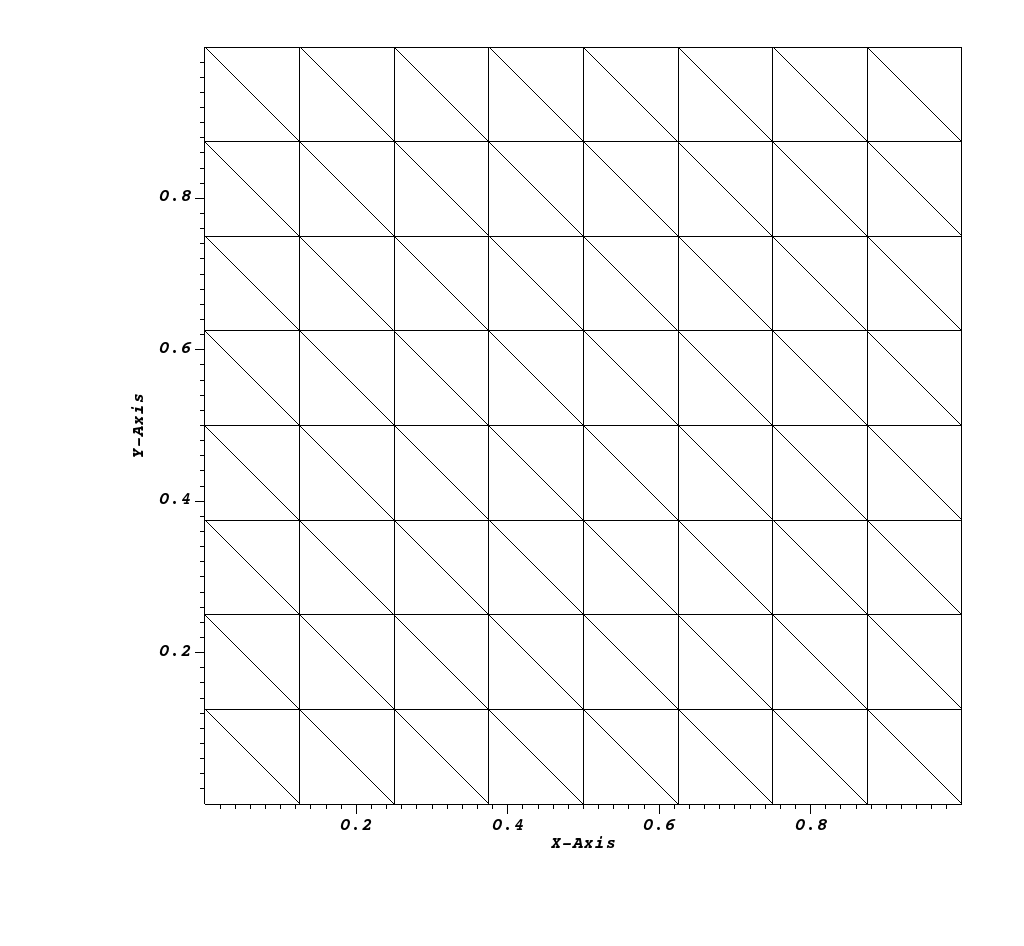
\includegraphics[width=\linewidth]{fig/mesh-2D.png}
        \caption{\small $h=\frac{1}{8}$ 时的计算网格}
    \end{minipage}
    \hfill
    \begin{minipage}[t]{0.4\textwidth}
        \centering
        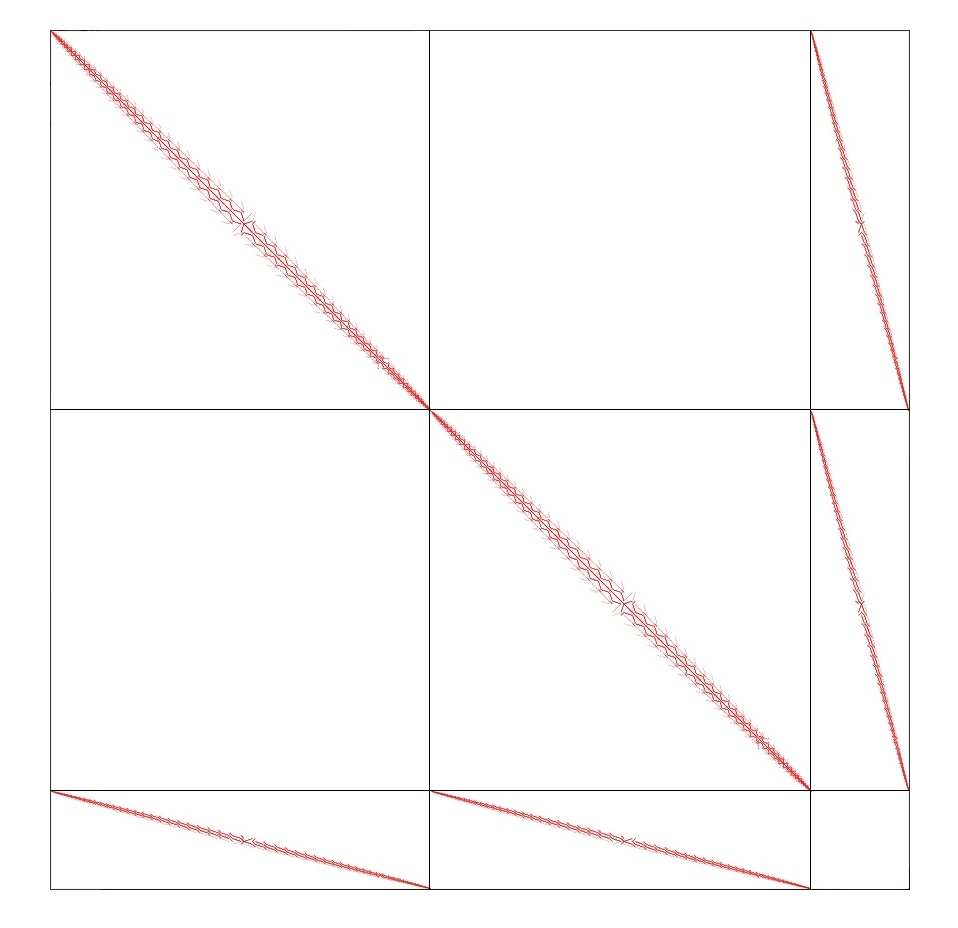
\includegraphics[width=\linewidth]{fig/sparsity-pattern-5.png}
        \caption{\small $h=\frac{1}{32}$ 时离散系统的稀疏模式}
    \end{minipage}
\end{figure}

\subsubsection{MINRES 方法}

按照题目要求, 我们使用 MINRES 方法求解, \verb|deal.ii| 中为我们提供了
\verb|SolverMinRes|, 可直接调用. 现在考虑题目所述的预优算子: 
\begin{equation}
    B=\begin{pmatrix}
        B_\Delta & &\\
        & B_\Delta &\\
        & & (\text{diag}\; M_Q)^{-1}
    \end{pmatrix}.
\end{equation}
其中 $B_\Delta$ 是使用多重网格 V-cycle 进行一轮松弛. 

考虑到 $\mathcal{P}_2$ 元的
索引非常复杂, 粗细网格插值极其困难, 因此我们决定使用代数多重网格 (AMG). 
\verb|Trilinos| 为我们提供了相关的库, \verb|deal.ii| 将其引入并进行了
用户友好的封装, 我们直接调用 \verb|TrilinosWrappers::PreconditionAMG| 即可. 
并且可以设置 \verb|higher_order_elements| 参数为 \verb|true|, 
从而对高阶有限元提供更好的支持. 另外, 我们也测试了将 $B_\Delta$ 设置为
多重网格 W-cycle 的一轮松弛, 测试结果见后文.

最后, 我们还需要计算误差. 我们采用 $n=3$ 的高斯求积公式
(二维情形下, 每个三角形中有 9 个积分节点, 具有 5 阶代数精度)
来近似计算误差的 $L^2$ 范数. 

\subsubsection{Uzawa 方法}

Uzawa 方法对速度与压强进行轮流更新, 即, 重复如下两步迭代:

(Uzawa-1) $\mathbf{u} \gets A^{-1}(\mathbf{f}-B'p)$;

(Uzawa-2) $p \gets p + M_Q^{-1}B\mathbf{u}$.

从实用角度出发, 我们更愿意使用非精确的 Uzawa 方法. 
即: 将上述迭代中的
$A^{-1}$ 用一轮多重网格 W-Cycle 松弛替代, 
将 $M_Q^{-1}$ 用 $(\text{diag}\; M_Q)^{-1}$ 替代. 
可以证明, 精确与非精确的 Uzawa 方法具有一样好的收敛性.
 其中, 非精确 Uzawa 的证明要更加困难, 
不过在实际使用中往往比精确 Uzawa 的表现更好.

\subsection{编译说明}

请安装依赖库: 
\begin{itemize}
    \item \verb|openMPI|(也可以用 \verb|MPICH| 等其它 MPI 软件包代替); 
    \item \verb|Trilinos| (\verb|deal.ii| 的 README 中提及了安装方式); 
    \item \verb|deal.ii| (请确保 \verb|DEAL_II_WITH_TRILINOS| 开关是开启状态). 
\end{itemize}

在确保依赖库正确安装后, 请输入以下命令编译. 
\begin{lstlisting}
cd src
mkdir build
cd build
cmake ..
make release
make
\end{lstlisting}
等待编译完成后, 用以下命令执行测试: 
\begin{lstlisting}
./stokes
\end{lstlisting}
上述测试将从 $h=\frac{1}{4}$ 开始, 逐次加密, 
一直运行到 $h=\frac{1}{1024}$. 

\subsection{测试结果}

\begin{figure}[H]
    \centering
    \begin{minipage}[t]{0.32\textwidth}
        \centering
        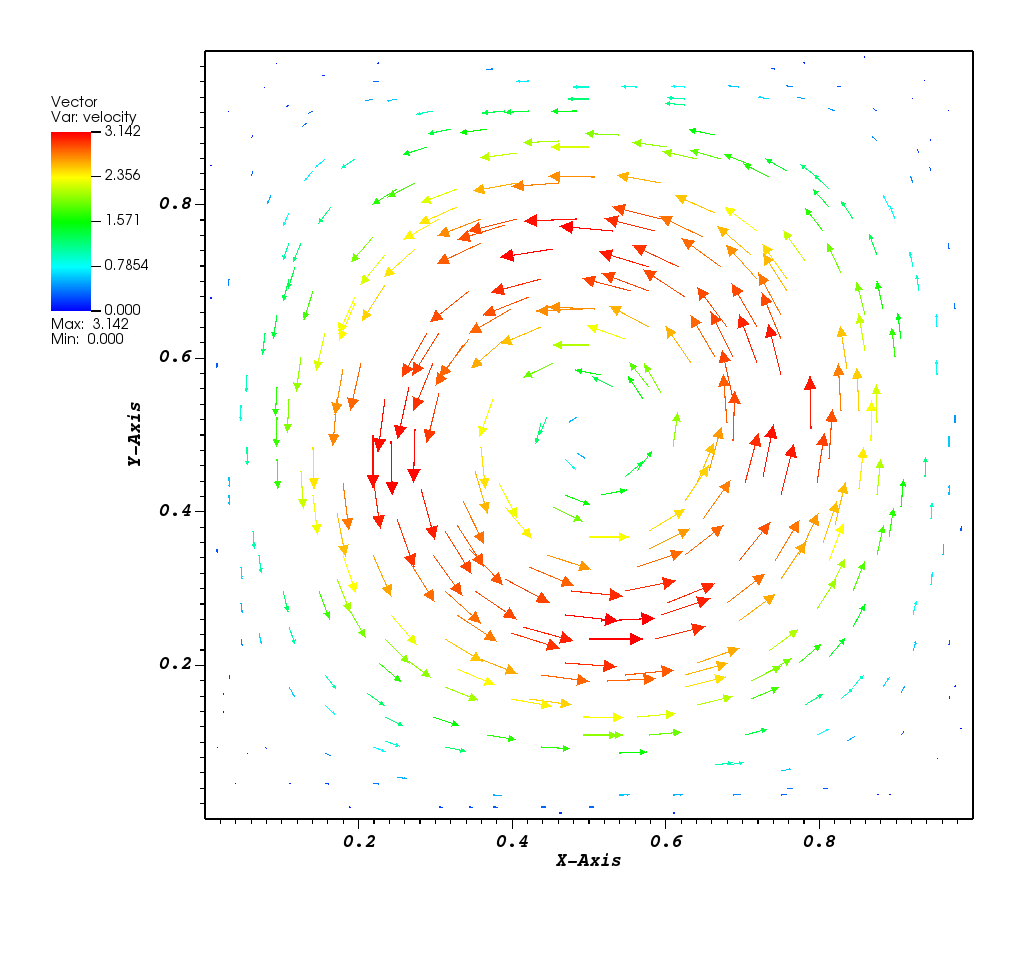
\includegraphics[width=\linewidth]{fig/velocity.png}
        \caption{\small $h=\frac{1}{256}$, 速度场}
    \end{minipage}
    \hfill
    \begin{minipage}[t]{0.32\textwidth}
        \centering
        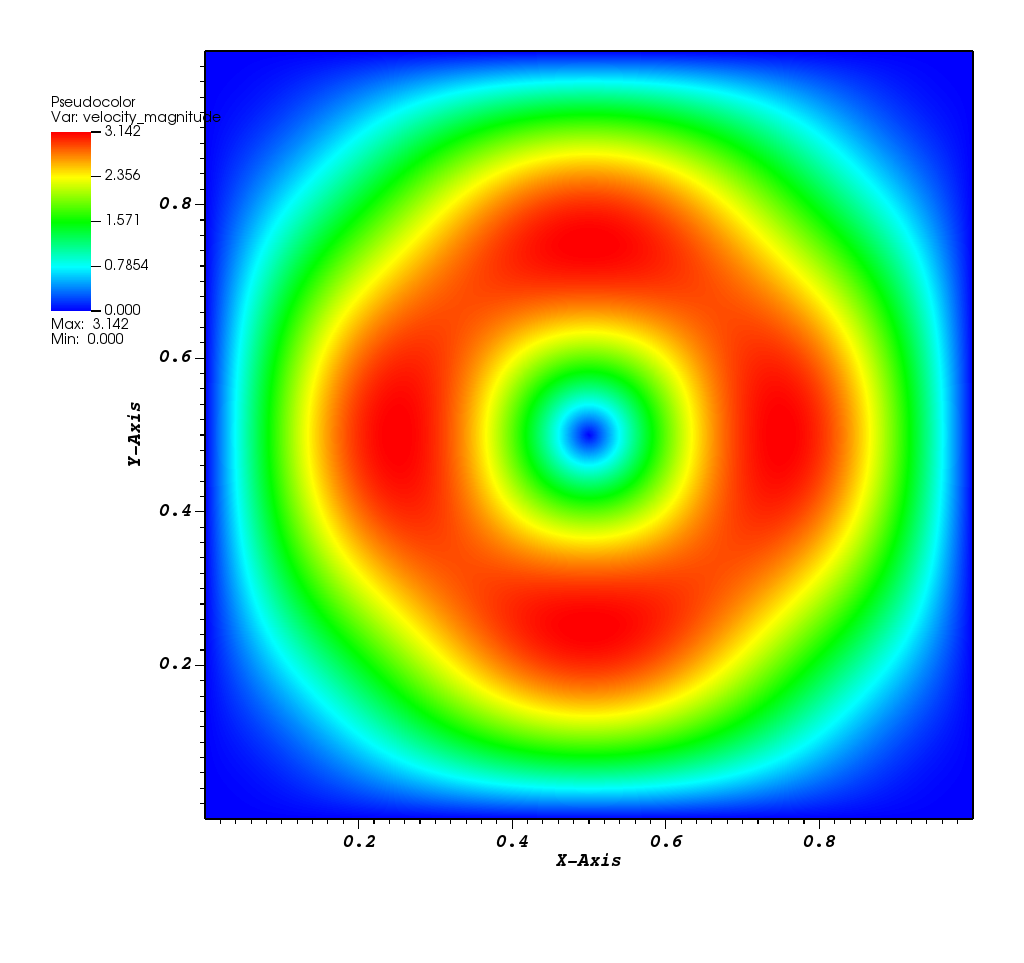
\includegraphics[width=\linewidth]{fig/velocity_mag.png}
        \caption{\small $h=\frac{1}{256}$, 速度的大小 $|\mathbf{u}|$}
    \end{minipage}
    \hfill
    \begin{minipage}[t]{0.32\textwidth}
        \centering
        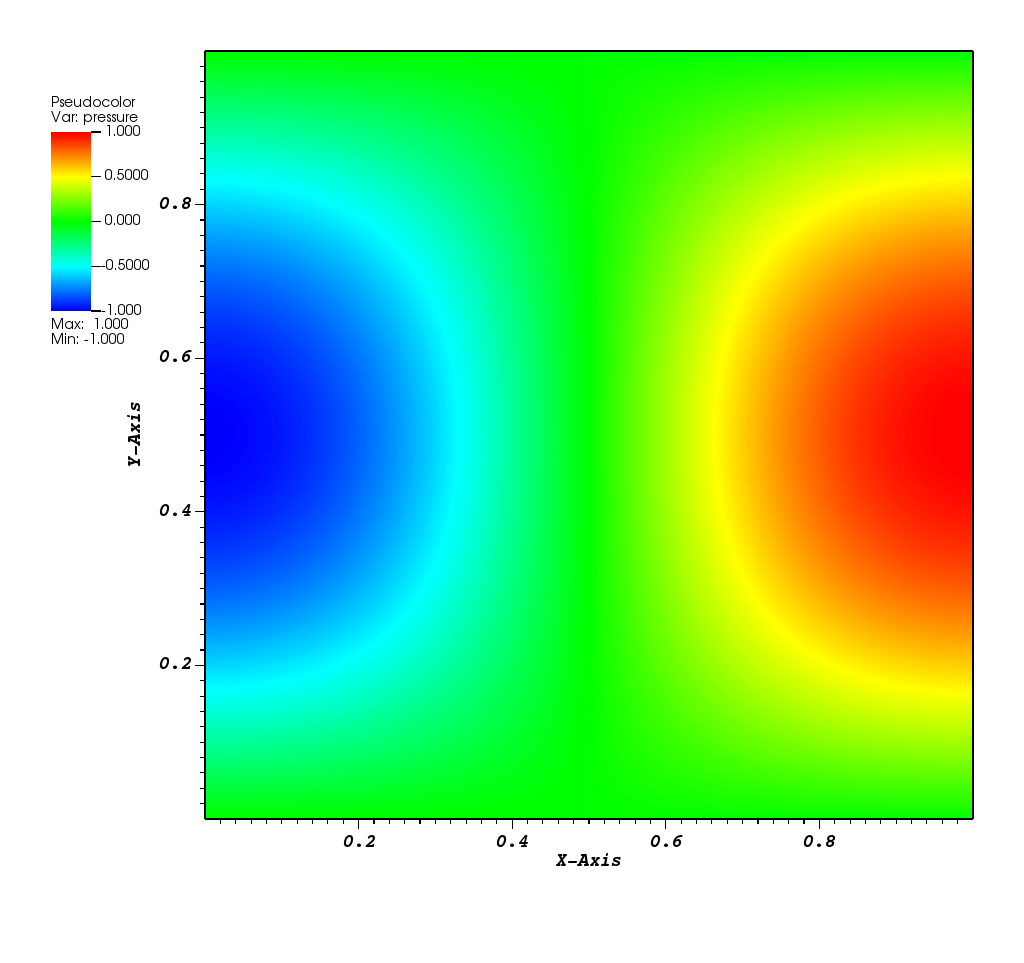
\includegraphics[width=\linewidth]{fig/pressure.png}
        \caption{\small $h=\frac{1}{256}$, 压强 $p$}
    \end{minipage}
\end{figure}

我们将求得的数值解用 \verb|VisIt| 绘制, 如图 $3-5$ 所示, 
其图像与我们构造的解析解一致. 

用朴素 MINRES 方法与预优 MINRES 方法对比, 见表1. 
表中的 “装配耗时” 是指从稀疏模式生成完毕开始, 到刚度矩阵计算完成耗费的时间; 
“求解耗时”是指 AMG 初始化和 MINRES 迭代的耗时之和. 
可以看到朴素 MINRES 方法的迭代次数随着网格加密而指数增长, 
求解时间也逐渐变得令人难以接受; 
而预优 MINRES 方法的迭代次数涨幅非常小, 
求解时间明显快于朴素 MINRES 方法, 
甚至对 $h=\frac{1}{1024}$ 的网格也能轻松求解. 
Uzawa 方法的迭代次数不随网格加密而增加, 效率最高.

此外, 我们还输出了预优 MINRES 方法求解误差的 $L^2$ 范数, 
见表2. 可以看到 $\mathbf{u}$ 保持了 $\mathcal{P}_2$ 元的
$L^2$ 范数三阶收敛性质; $p$ 保持了 $\mathcal{P}_1$ 元的
$L^2$ 范数二阶收敛性质. 

% Please add the following required packages to your document preamble:
% \usepackage{multirow}
\begin{table}[H]
    \centering
    \begin{tabular}{c|ccccc}
    \hline
                                        & $h$               & $\frac{1}{128}$  & $\frac{1}{256}$ & $\frac{1}{512}$  & $\frac{1}{1024}$ \\ \hline
    \multirow{3}{*}{\begin{tabular}[c]{@{}c@{}} Uzawa 方法 \\ (多重网格采用W-Cycle)\end{tabular}}    
                                       & 装配耗时 (s)     &   0.076   & 0.305            &   1.22   &  4.87              \\
                                        & 求解耗时 (s)       &   0.76   & 3.30            &   14.9   &  60.9              \\
                                        & UZAWA 迭代次数        &   60   & 59             &   59   &  59             \\ \hline
    \multirow{3}{*}{\begin{tabular}[c]{@{}c@{}} 预优 MINRES 方法 \\ (多重网格采用W-Cycle)\end{tabular}}    
                                        & 装配耗时 (s)     &   0.121   & 0.482            &   1.94   &  7.85              \\
                                        & 求解耗时 (s)       &   0.73   & 3.62            &   16.7   &   75.5             \\
                                        & MINRES 迭代次数        &   68   & 71             &   75   &  78             \\ \hline
    \multirow{3}{*}{\begin{tabular}[c]{@{}c@{}} 预优 MINRES 方法 \\ (多重网格采用V-Cycle)\end{tabular}}    
                                        & 装配耗时 (s)     &   0.122   & 0.49            &   1.96   &  7.77              \\
                                        & 求解耗时 (s)       &   0.73   & 3.92            &   18.9   &  86.7              \\
                                        & MINRES 迭代次数        &   80   & 85             &   100   &  105             \\ \hline
    \multirow{3}{*}{朴素 MINRES 方法} & 装配耗时 (s)        &  0.168    & 0.601         &  2.37    &  9.59             \\
                                    & 求解耗时 (s)         &   9.61   &   93.5     &   791   &    >1h, killed   \\
                                    & MINRES 迭代次数          &   2898   &  5449     &   10628   &                \\ \hline
    \end{tabular}
    \caption{\small MINRES 方法与 Uzawa 方法, $h=\frac{1}{128}$ 到 $\frac{1}{1024}$ 的 CPU 耗时. 迭代终止条件均为残差的 $2$ 范数小于等于右端项 $2$ 范数的 $10^{-6}$ 倍, 即 $||\text{res}||_2\leq 10^{-6}||\text{rhs}||_2$. }
\end{table}

\vspace{-1em}
\begin{table}[H]
    \centering
    \begin{tabular}{cccccc}
    \hline
         $h$               & $\frac{1}{256}$ & 收敛阶  & $\frac{1}{512}$ & 收敛阶  & $\frac{1}{1024}$ \\ \hline
         $||u_1^h-u_1||_{L^2}$ & 2.03e-07        & 3.00 & 2.54e-08        & 2.98 & 3.23e-09         \\
         $||u_2^h-u_2||_{L^2}$ & 2.03e-07        & 2.99 & 2.55e-08        & 2.97 & 3.25e-09         \\
         $||p^h-p||_{L^2}$     & 6.30e-06        & 1.99 & 1.59e-06        & 1.96 & 4.08e-07         \\ \hline
    \end{tabular}
    \caption{\small 预优 MINRES 方法 (多重网格采用W-Cycle), $h=\frac{1}{256}$ 到 $\frac{1}{1024}$ 的 $L^2$ 误差}
\end{table}

\vspace{-2em}
\section{题外话: 投影方法}
\vspace{-0.5em}

事实上, 假如我们额外地知道 $\Delta \mathbf{u}$ 在边界上的法向分量, 
我们可以使用投影方法来解决 Stokes 方程. 
只需对 Stokes 方程两侧应用散度算子, 然后将不可压条件代入即可. 
第一步是求解 Neumann 边界条件的 Poisson 方程: 
\begin{equation}
    \left\{
        \begin{array}{ll}
            \Delta p = \nabla \cdot \mathbf{f}& ,\text{in}\;\Omega,\\
            \mathbf{n}\cdot\nabla p = \mathbf{n}\cdot(\mathbf{f}+\Delta\mathbf{u}) & ,\text{on}\;\partial \Omega.
        \end{array}
    \right.
\end{equation}
这里我们并不需要真的去计算 $\nabla \cdot \mathbf{f}$, 因为在弱形式下, 我们有: 
\begin{equation}
    (\nabla p,\nabla q)_\Omega=(\mathbf{f},\nabla q)_\Omega+(\mathbf{n}\cdot\Delta\mathbf{u},q)_{\partial \Omega}.
\end{equation}
第二步是计算 $\mathbf{u}=\mathbf{f}-\nabla p$, 
然后第三步是解 $u_1$ 与 $u_2$ 的齐次 Dirichlet 边界条件 Poisson 方程. 

投影法的优势在于速度快, 而且 $\mathbf{u}$ 与 $p$ 可以使用一样的有限元, 
从而拥有一致的高阶收敛阶. 我们用 $\mathcal{Q}_2$ 元实现了 Stokes 方程的
投影法, 表3展示了投影法的误差和 CPU 耗时.
\begin{table}[H]
    \centering
    \begin{tabular}{cccccc}
    \hline
         $h$               & $\frac{1}{256}$ & 收敛阶  & $\frac{1}{512}$ & 收敛阶  & $\frac{1}{1024}$ \\ \hline
         $||u_1^h-u_1||_{L^2}$ & 1.12e-07        & 3.00 & 1.40e-08        & 2.96 & 1.80e-09         \\
         $||u_2^h-u_2||_{L^2}$ & 1.12e-07        & 3.00 & 1.40e-08        & 2.95 & 1.81e-09         \\
         $||p^h-p||_{L^2}$     & 7.04e-09        & 3.12 & 8.10e-10        & 3.03 & 9.93e-11         \\
         CPU 耗时 (s)          & 2.45        &    & 10.4        &  & 43.1         \\ \hline
    \end{tabular}
    \caption{\small 投影法, $h=\frac{1}{256}$ 到 $\frac{1}{1024}$ 的 $L^2$ 误差、CPU 耗时}
\end{table}

\appendix
%\appendixpage
\addappheadtotoc

\end{document}
